\documentclass{standalone}
\usepackage{tikz}
\usetikzlibrary{calc}
\begin{document}
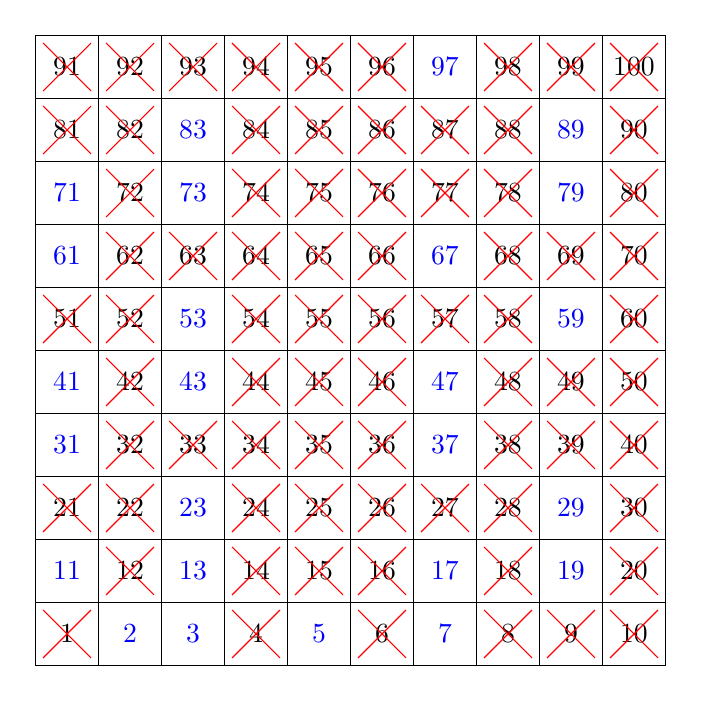
\begin{tikzpicture}[scale=0.8]
\foreach \x in {0,...,9} {
    \foreach \y in {1,...,10} {
        \draw (\x,\y) + (-0.5cm,-0.5cm) rectangle ++ (0.5cm,0.5cm);
        \pgfmathtruncatemacro{\nb}{\x*10+\y}
        \ifnum\nb=1
            \node[minimum size=1cm] (last) at (\y-1,\x+1) {\nb};
            \def\pgfmathresult{0}
        \else
            \pgfmathisprime{\nb}
            \ifnum\pgfmathresult=1
                \node[minimum size=1cm, blue] (last) at (\y-1,\x+1) {\nb};
            \else
                \node[minimum size=1cm] (last) at (\y-1,\x+1) {\nb};
            \fi
        \fi
        \ifnum\pgfmathresult=0
            \draw[red] ($(last.north west)!0.4!(last.center)$) -- ($(last.center)!0.6!(last.south east)$);
            \draw[red] ($(last.north east)!0.4!(last.center)$) -- ($(last.center)!0.6!(last.south west)$);
        \fi
    }
}
\end{tikzpicture}
\end{document}
